\documentclass{article}

\usepackage{graphicx}
\usepackage[a4paper, total={18cm, 26.7cm}]{geometry}
\usepackage{helvet}

\renewcommand{\familydefault}{\sfdefault}

\pagenumbering{gobble}

\newcommand{\job}[4]{
\vspace{0.5em}
\noindent
\begin{tabular}{ p{0.75\textwidth} l }

\textbf{#2} 

\textit{#3} 

#4 
&
#1
\\
\end{tabular}
\noindent
}

\newcommand{\degree}[3]{
\noindent
\textbf{#1}

#2, #3

\vspace{12pt}
}

\begin{document}

\noindent%
\begin{minipage}{.70\textwidth}

\section*{Hannu Leppinen}

\begin{tabular}{ l l }
Address: & Pellavakaski 12 B, 02340 Espoo, Finland \\
E-mail:  & hannu.leppinen@gmail.com \\
Phone:	 & +358 50 596 3888
\end{tabular}

\section*{Summary}

An embedded software engineer with several years of experience in developer, technical lead, and architect roles.
Has delivered critical embedded software in C and Ada on bare metal, real-time operating systems, and Linux.
Has also developed supporting tools and frameworks in Python and Java.
Has also led developers working on critical embedded software while being responsible for the overall software architecture,
technical quality, and communication with project stakeholders and customers.

\end{minipage}%
\hfill
\begin{minipage}{.22\textwidth}

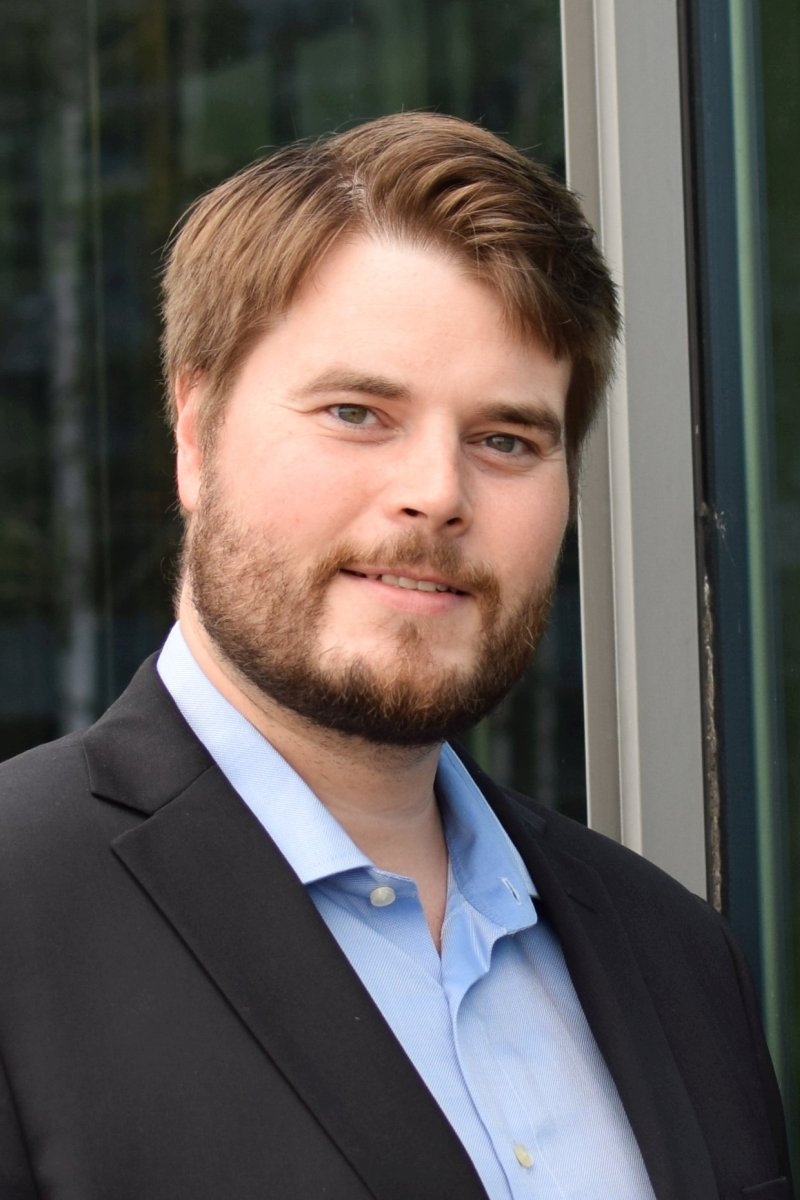
\includegraphics[width=\textwidth]{cv_profile}

\end{minipage}%

\vspace{1cm}

\noindent%
\begin{minipage}[t]{.65\textwidth}

\section*{Work Experience}

\job{08/2020 -- Present}{Software Design Lead}{Huld, Espoo, Finland}{
Lead developer and architect in the PLATO space telescope spacecraft control software project. The software will control the telescope once in orbit.
}

\job{02/2015 -- 08/2020}{Software Engineer}{Space Systems Finland, Espoo, Finland}{
Software engineer in several spacecraft software projects (critical embedded software).
}

\job{03/2017 -- 11/2017}{Software Engineer}{Airbus Defence and Space, Stevenage, UK}{
Software consultant in the ExoMars rover control software project. The software will control the rover on the surface of Mars.
}

\job{04/2013 -- 02/2015}{Software Engineer}{ICEYE, Espoo, Finland}{
Early on-board software work and team leading for the ICEYE satellites (while still a project at Aalto University). Also some limited hardware design and component selection duties.
}

\job{06/2012 -- 02/2015}{Researcher}{Aalto University, Espoo, Finland}{
Researcher in the Aalto-1 satellite project, including software and hardware design work. The Aalto-1 satellite runs embedded Linux.
}

\job{07/2011 -- 10/2011}{Student Software Engineer}{European Space Agency Summer of Code in Space, Noordwijk, NL}{
Implementing spacecraft attitude dynamics into the OpenSimKit simulator.
}

\job{05/2011 -- 08/2011}{Software Test Engineer Trainee}{ABB, Helsinki, Finland}{
Testing and development of control software for variable-frequency drives.
}

\end{minipage}%
\hfill
\begin{minipage}[t]{.22\textwidth}

\section*{Skills}

\subsubsection*{Programming}

C, Ada, Python, MATLAB, Java,  C++, Simulink

\subsubsection*{Embedded}

RTEMS, FreeRTOS, Bare metal, Embedded Linux, SPARC processors, ARM processors, UART, SPI, I2C, CAN bus

\subsubsection*{Other}

Git, Jira, GitLab, Docker, Linux, Windows

\section*{Education}

\degree{Doctoral degree in Space Science and Technology}{Aalto University}{2018}

\degree{Master's degree in Automation and Systems Technology}{Aalto University}{2013}

\degree{Bachelor's degree in Automation and Systems Technology}{Aalto University}{2011}

\end{minipage}%

\end{document} 
